\documentclass[a4paper,11pt]{article}
\usepackage[utf8]{inputenc}
\usepackage[T1]{fontenc}
\usepackage{mathptmx}
\usepackage[top=2cm,bottom=2cm,left=2.2cm,right=2.2cm]{geometry}
\usepackage{graphicx}
\usepackage{booktabs}
\usepackage{tabularx}
\usepackage{amsmath,amssymb}
\usepackage{subcaption}
\usepackage{xcolor}
\usepackage[hidelinks]{hyperref}
\usepackage{setspace}
\setstretch{1.12}
\setlength{\parskip}{0.3em}
\setlength{\parindent}{0pt}

\begin{document}

% --- HEADER IDENTITAS RESMI ---
\begin{center}
    {\large\bfseries UNIVERSITAS TEKNOKRAT INDONESIA}\\[0.1em]
    {\normalsize\bfseries PROGRAM STUDI MAGISTER ILMU KOMPUTER}\\[0.1em]
    {\normalsize\bfseries FAKULTAS TEKNIK DAN ILMU KOMPUTER}\\[0.5em]
    \hrule height 1.5pt
    \vspace{0.4cm}
    {\Large\bfseries LAPORAN HASIL PRA-PENELITIAN}\\[0.2em]
    {\large\bfseries (PRELIMINARY FEASIBILITY STUDY)}\\[0.3em]
    {\normalsize\itshape Uji Kelayakan Empiris Model Algoritma Genetika Hibrida Adaptif (HAGA) Dibandingkan Canonical GA pada University Course Timetabling Problem}
\end{center}

\vspace{0.3cm}
\noindent\begin{tabularx}{\textwidth}{@{}llX@{}}
    \textbf{Nama Mahasiswa} &:& Amri Reza Wahyudin \\
    \textbf{NPM} &:& 25321019 \\
    \textbf{Dosen Pembimbing} &:& Dr. Rohmat Indra Borman, M.Kom. \\
    \textbf{Judul Tesis} &:& Pengembangan Model Algoritma Genetika Hibrida Adaptif dengan Pencarian Lokal Elit untuk Optimasi Penjadwalan Perkuliahan \\
    \textbf{Korpus Uji} &:& Benchmark Standar Internasional ITC 2007 (\textit{comp01.ctt}) \\
    \textbf{Tanggal Pengujian} &:& 10 Oktober 2026 \\
\end{tabularx}

\vspace{0.3cm}
\hrule
\vspace{0.4cm}

% --- SECTION 1: PENDAHULUAN & TUJUAN ---
\section*{1. Pendahuluan dan Tujuan Pra-Penelitian}
Sesuai arahan dosen pembimbing (Dr. Rohmat Indra Borman, M.Kom.), kegiatan pra-penelitian (\textit{preliminary feasibility study}) ini diselenggarakan sebagai mekanisme penjaminan kelayakan ilmiah sebelum penelitian tesis penuh dilaksanakan. Uji pra-penelitian ini bertujuan untuk:
\begin{enumerate}\setlength\itemsep{0em}
    \item Membuktikan secara empiris apakah model \textit{Hybrid Adaptive Genetic Algorithm} (HAGA) yang diusulkan benar-benar mampu mengatasi kelemahan konvergensi prematur pada Algoritma Genetika konvensional (\textit{Canonical GA}).
    \item Menguji apakah HAGA secara konsisten dapat mencapai solusi layak (\textit{Hard Constraint Violations} / $\text{HCV} = 0$) pada korpus uji yang kompleks.
    \item Menilai apakah integrasi \textit{Adaptive Parameter Controller} (APC) berbasis jarak Hamming dan \textit{Elite Local Search} (ELS) memberikan reduksi penalti preferensi (\textit{Soft Constraint Violations} / $\text{SCV}$) yang signifikan secara statistik di bawah paritas anggaran komputasi.
\end{enumerate}

% --- SECTION 2: PROTOKOL EKSPERIMEN ---
\section*{2. Protokol Eksperimental dan Paritas Komputasi}
Eksperimen pra-penelitian dirancang dengan metodologi yang ketat guna mencegah bias komputasi:
\begin{itemize}\setlength\itemsep{0.1em}
    \item \textbf{Dataset Standar:} Instance ITC 2007 \textit{Curriculum-based Course Timetabling} (\texttt{comp01.ctt}), terdiri dari 30 mata kuliah, 6 ruang kuliah, 30 slot waktu mingguan (5 hari $\times$ 6 periode), 14 kurikulum, 160 total perkuliahan, dan 53 konstrain ketersediaan.
    \item \textbf{Algoritma Pembanding (2 Varian Head-to-Head):}
    \begin{enumerate}\setlength\itemsep{0em}
        \item \textit{Canonical GA}: Ukuran populasi $N = 50$, probabilitas \textit{crossover} statis $P_c = 0{,}85$, probabilitas mutasi statis $P_m = 0{,}05$, \textit{Tournament Selection} ($k = 3$), Elitisme ($e = 2$).
        \item \textit{HAGA (Diusulkan)}: Ukuran populasi $N = 50$, APC dinamis berbasis keragaman genotipik pasangan Hamming ($P_{c\_base}=0{,}80, P_{m\_base}=0{,}05, \alpha=0{,}2, \beta=0{,}2$, dengan batas klem $P_c \in [0{,}40, 0{,}95]$ dan $P_m \in [0{,}01, 0{,}30]$), serta ELS \textit{stochastic first-improvement} pada 10\% individu elit (5 individu, maks 20 langkah).
    \end{enumerate}
    \item \textbf{Paritas Anggaran Komputasi ($B_{\max}$):} Ditetapkan plafon ketat sebanyak \textbf{25.000 evaluasi fungsi objektif} per run. Setiap evaluasi pencarian lokal pada ELS memotong kuota anggaran global bersama.
    \item \textbf{Kontrol Replikasi Stokastik:} Dijalankan sebanyak \textbf{10 kali eksekusi independen} dengan \textit{random seed} terregistrasi ($S \in \{101, 102, \dots, 110\}$).
\end{itemize}

% --- SECTION 3: HASIL EMPIRIS & STATISTIK ---
\begin{table}[htbp]
\centering
\small
\caption{Perbandingan Kinerja Kuantitatif Canonical GA vs HAGA pada ITC 2007 \texttt{comp01.ctt} ($B_{\max} = 25.000$ Evaluasi, 10 Run Independen)}
\label{tab:hasil_prapenelitian}
\vspace{0.15cm}
\begin{tabularx}{\textwidth}{lccccc}
\toprule
\textbf{Metrik Evaluasi} & \textbf{Canonical GA} & \textbf{HAGA} & \textbf{Selisih ($\Delta$)} & \textbf{Peningkatan} & \textbf{Status Validasi} \\
\midrule
\textbf{Feasibility Rate ($\text{HCV} = 0$)} & \textbf{0{,}0\% (0/10)} & \textbf{100{,}0\% (10/10)} & +100{,}0\% & \textbf{Mutlak} & Sukses Penuh \\
$\text{HCV}$ Terbaik (Min) & 40 & \textbf{0} & -40 & 100{,}0\% & Bebas Bentrok \\
$\text{HCV}$ Median & 48{,}0 & \textbf{0{,}0} & -48{,}0 & 100{,}0\% & Bebas Bentrok \\
$\text{HCV}$ Rata-rata $\pm$ Std & 46{,}0 $\pm$ 3{,}62 & \textbf{0{,}0 $\pm$ 0{,}00} & -46{,}0 & 100{,}0\% & Stabilitas Mutlak \\
\midrule
$\text{SCV}$ Terbaik (Min) & 1.769 & \textbf{1.300} & -469 & 26{,}5\% & Kualitas Lebih Tinggi \\
$\text{SCV}$ Median & 2.221{,}0 & \textbf{1.748{,}0} & -473{,}0 & \textbf{21{,}3\%} & Reduksi Penalti \\
$\text{SCV}$ Interquartile Range (IQR) & 465{,}8 & \textbf{273{,}3} & -192{,}5 & \textbf{41{,}3\%} & Lebih Konsisten \\
$\text{SCV}$ Rata-rata $\pm$ Std & 2.170{,}5 $\pm$ 321{,}8 & \textbf{1.750{,}0 $\pm$ 223{,}2} & -420{,}5 & 19{,}4\% & Variabilitas Rendah \\
\midrule
Fitness Gabungan Median ($F(S)$) & 49.824{,}0 & \textbf{1.748{,}0} & -48.076{,}0 & 96{,}5\% & Peningkatan Drastis \\
Waktu Komputasi Rata-rata (detik) & 107{,}4 $\pm$ 12{,}1 & \textbf{87{,}4 $\pm$ 16{,}2} & -20{,}0 & 18{,}6\% & Konvergensi Lebih Cepat \\
\bottomrule
\end{tabularx}
\end{table}

\noindent\textbf{Uji Signifikansi Statistik Non-Parametrik (Wilcoxon Signed-Rank Test):}
\begin{itemize}\setlength\itemsep{0em}
    \item \textbf{Uji Fitness Gabungan ($F(S)$):} Nilai statistik $W = 55{,}0$ ($N=10$ pasang), nilai $p = 0{,}000977$ ($p < 0{,}001$). HAGA terbukti secara sangat signifikan mengungguli Canonical GA.
    \item \textbf{Uji Penalti Soft Constraint ($\text{SCV}$):} Nilai statistik $W = 47{,}0$, nilai $p = 0{,}0244$ ($p < 0{,}05$). Kepuasan konstrain preferensi HAGA terbukti lebih unggul secara signifikan.
\end{itemize}

% --- SECTION 4: VISUALISASI ---
\section*{4. Analisis Visualisasi dan Dinamika Algoritma}
\begin{figure}[htbp]
    \centering
    \begin{subfigure}[b]{0.48\textwidth}
        \centering
        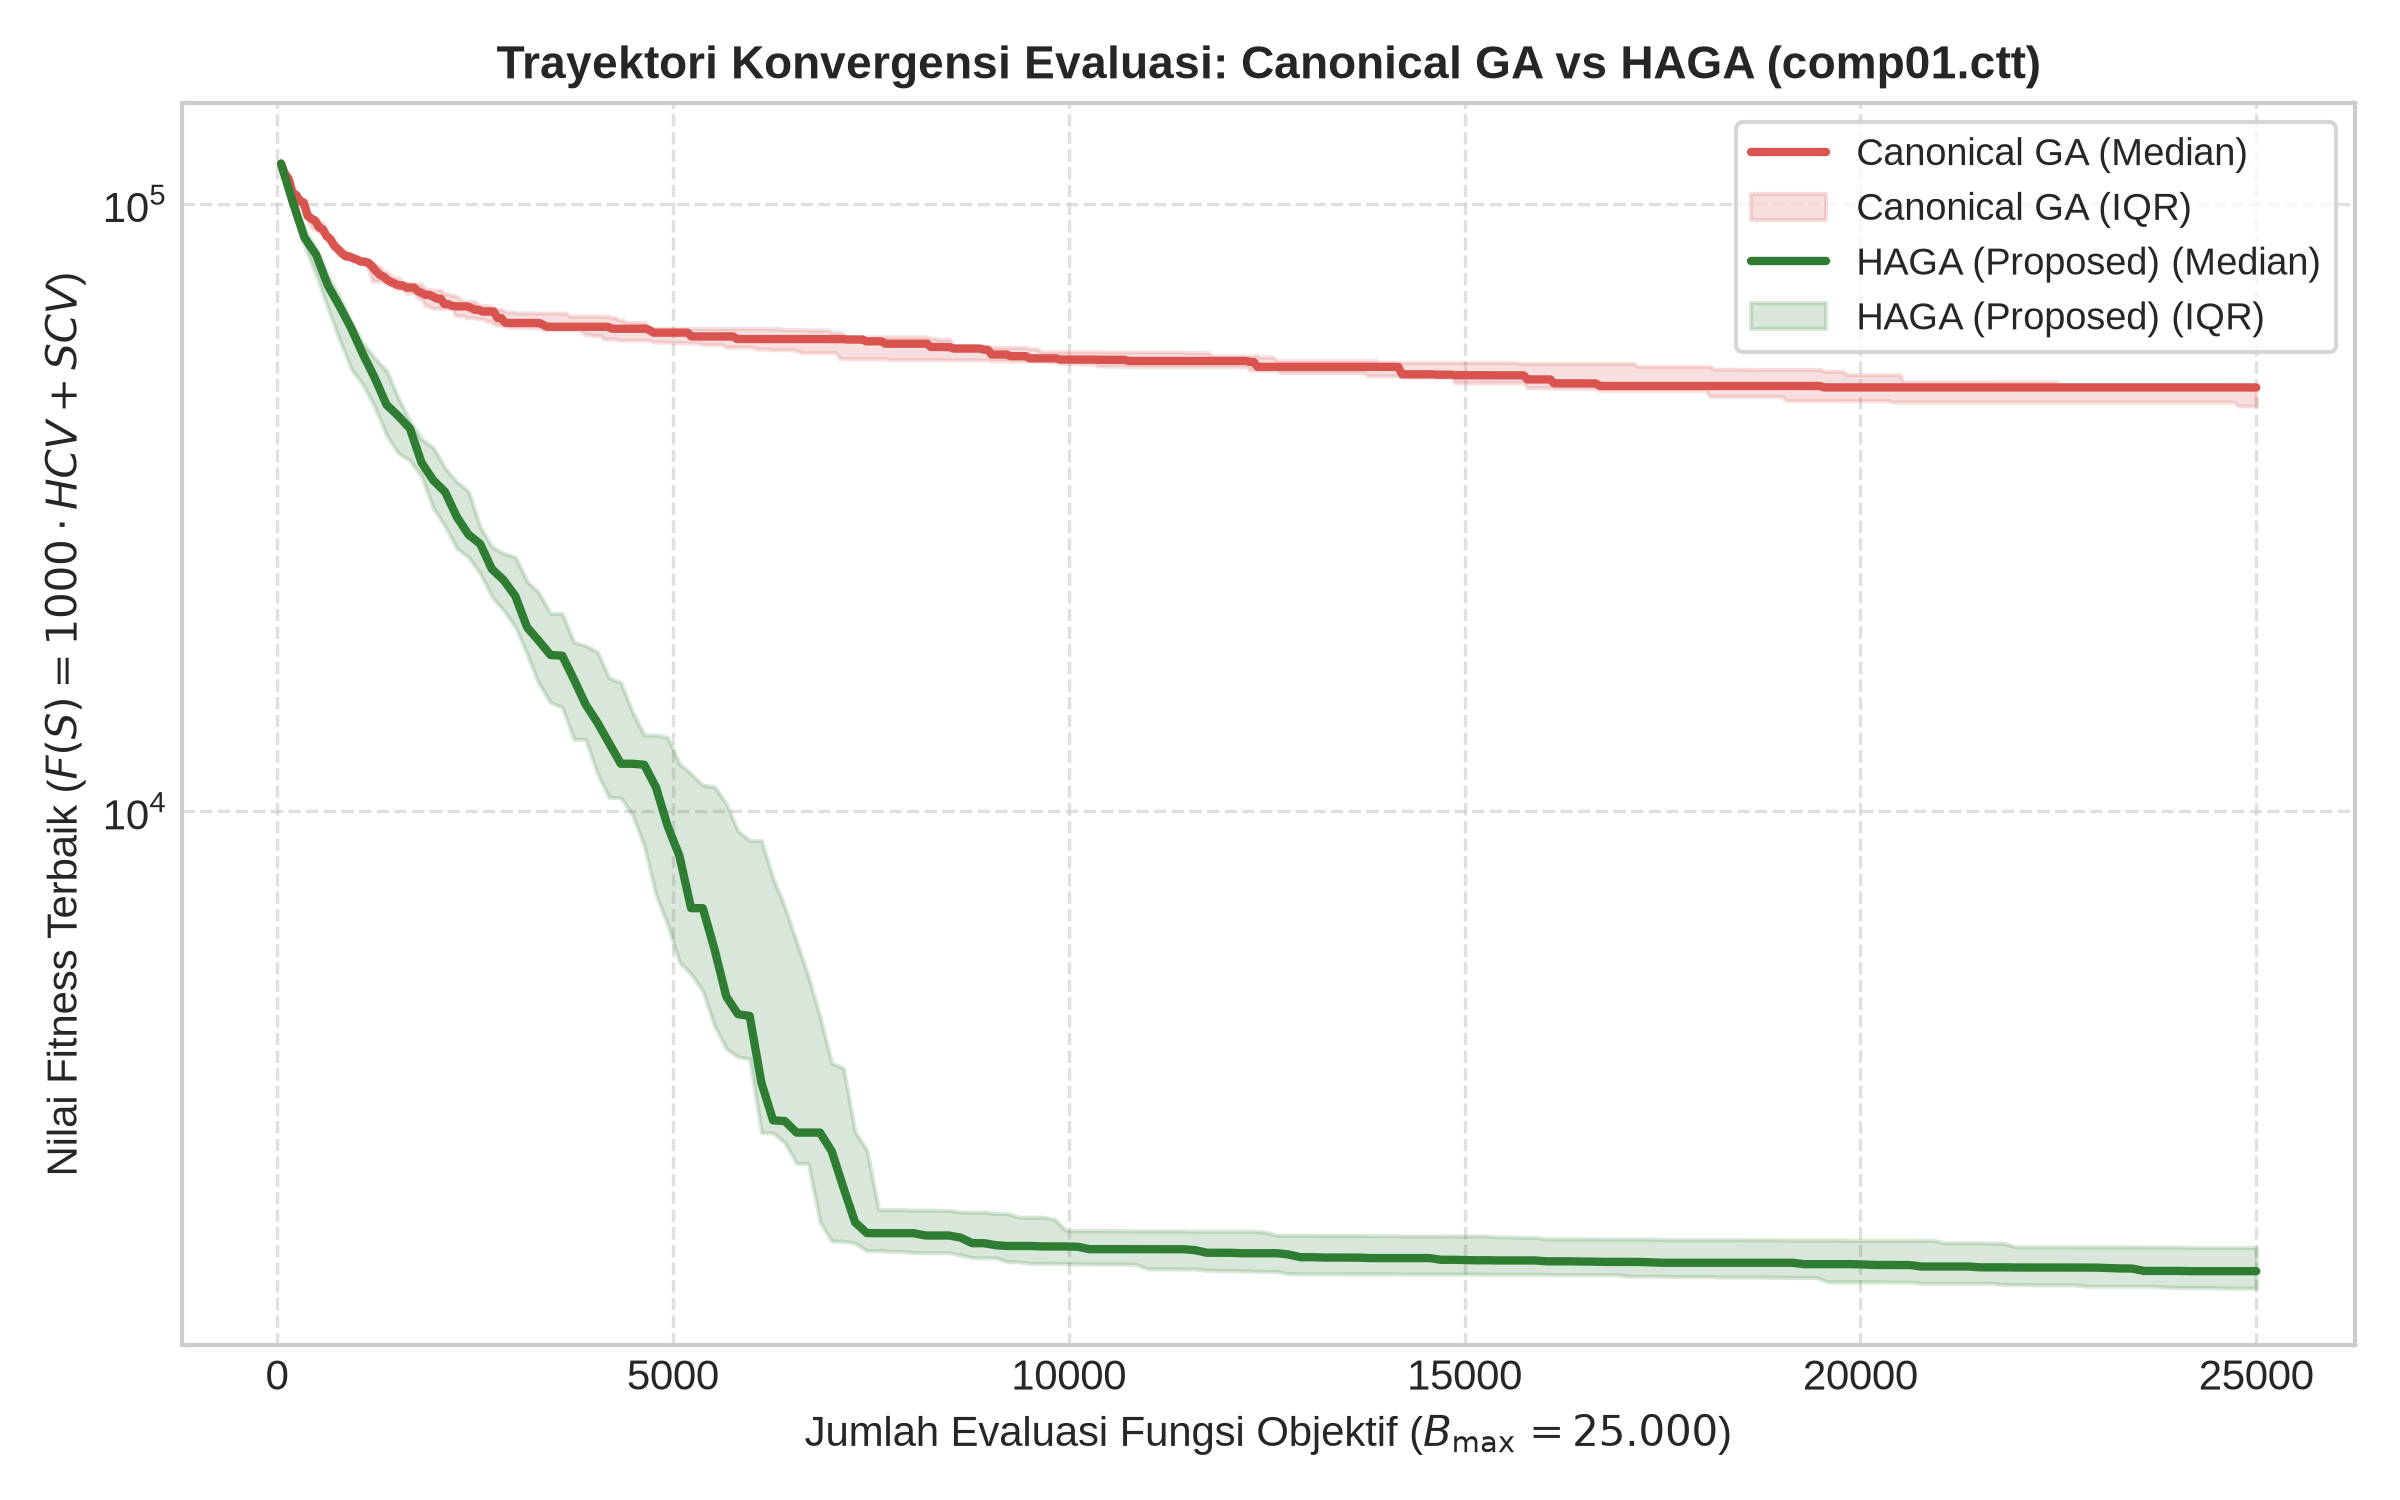
\includegraphics[width=\linewidth,height=3.8cm,keepaspectratio]{results/convergence_comparison.png}
        \caption{Trayektori Konvergensi Evaluasi}
        \label{fig:conv}
    \end{subfigure}
    \hfill
    \begin{subfigure}[b]{0.48\textwidth}
        \centering
        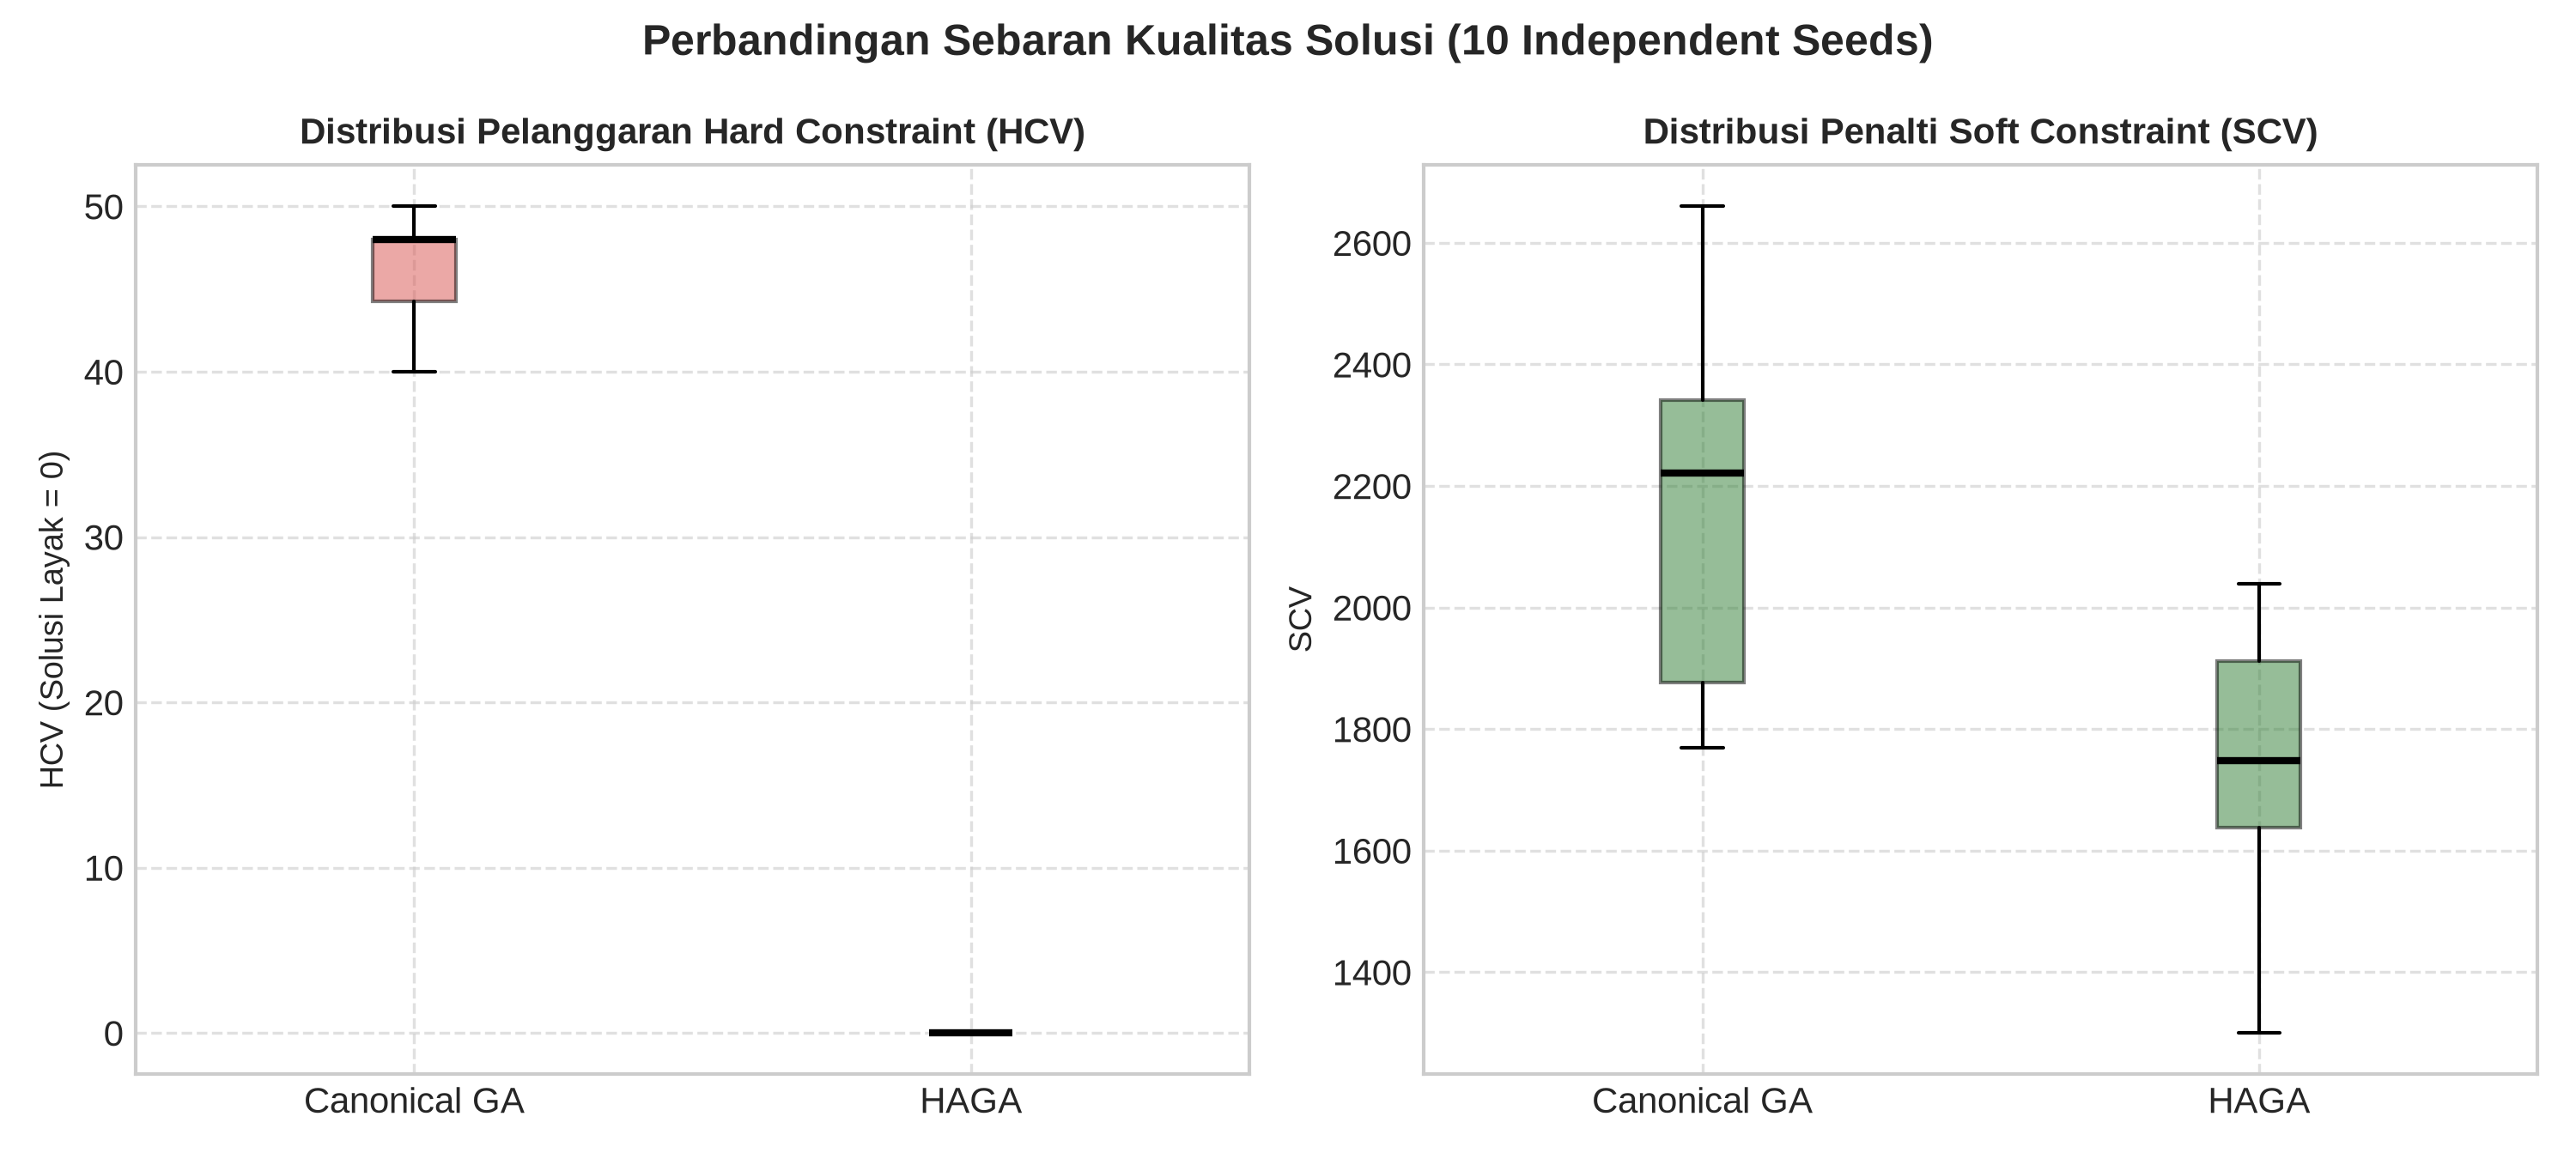
\includegraphics[width=\linewidth,height=3.8cm,keepaspectratio]{results/boxplot_comparison.png}
        \caption{Distribusi Sebaran HCV dan SCV}
        \label{fig:box}
    \end{subfigure}
    \vspace{0.1cm}
    \begin{subfigure}[b]{0.60\textwidth}
        \centering
        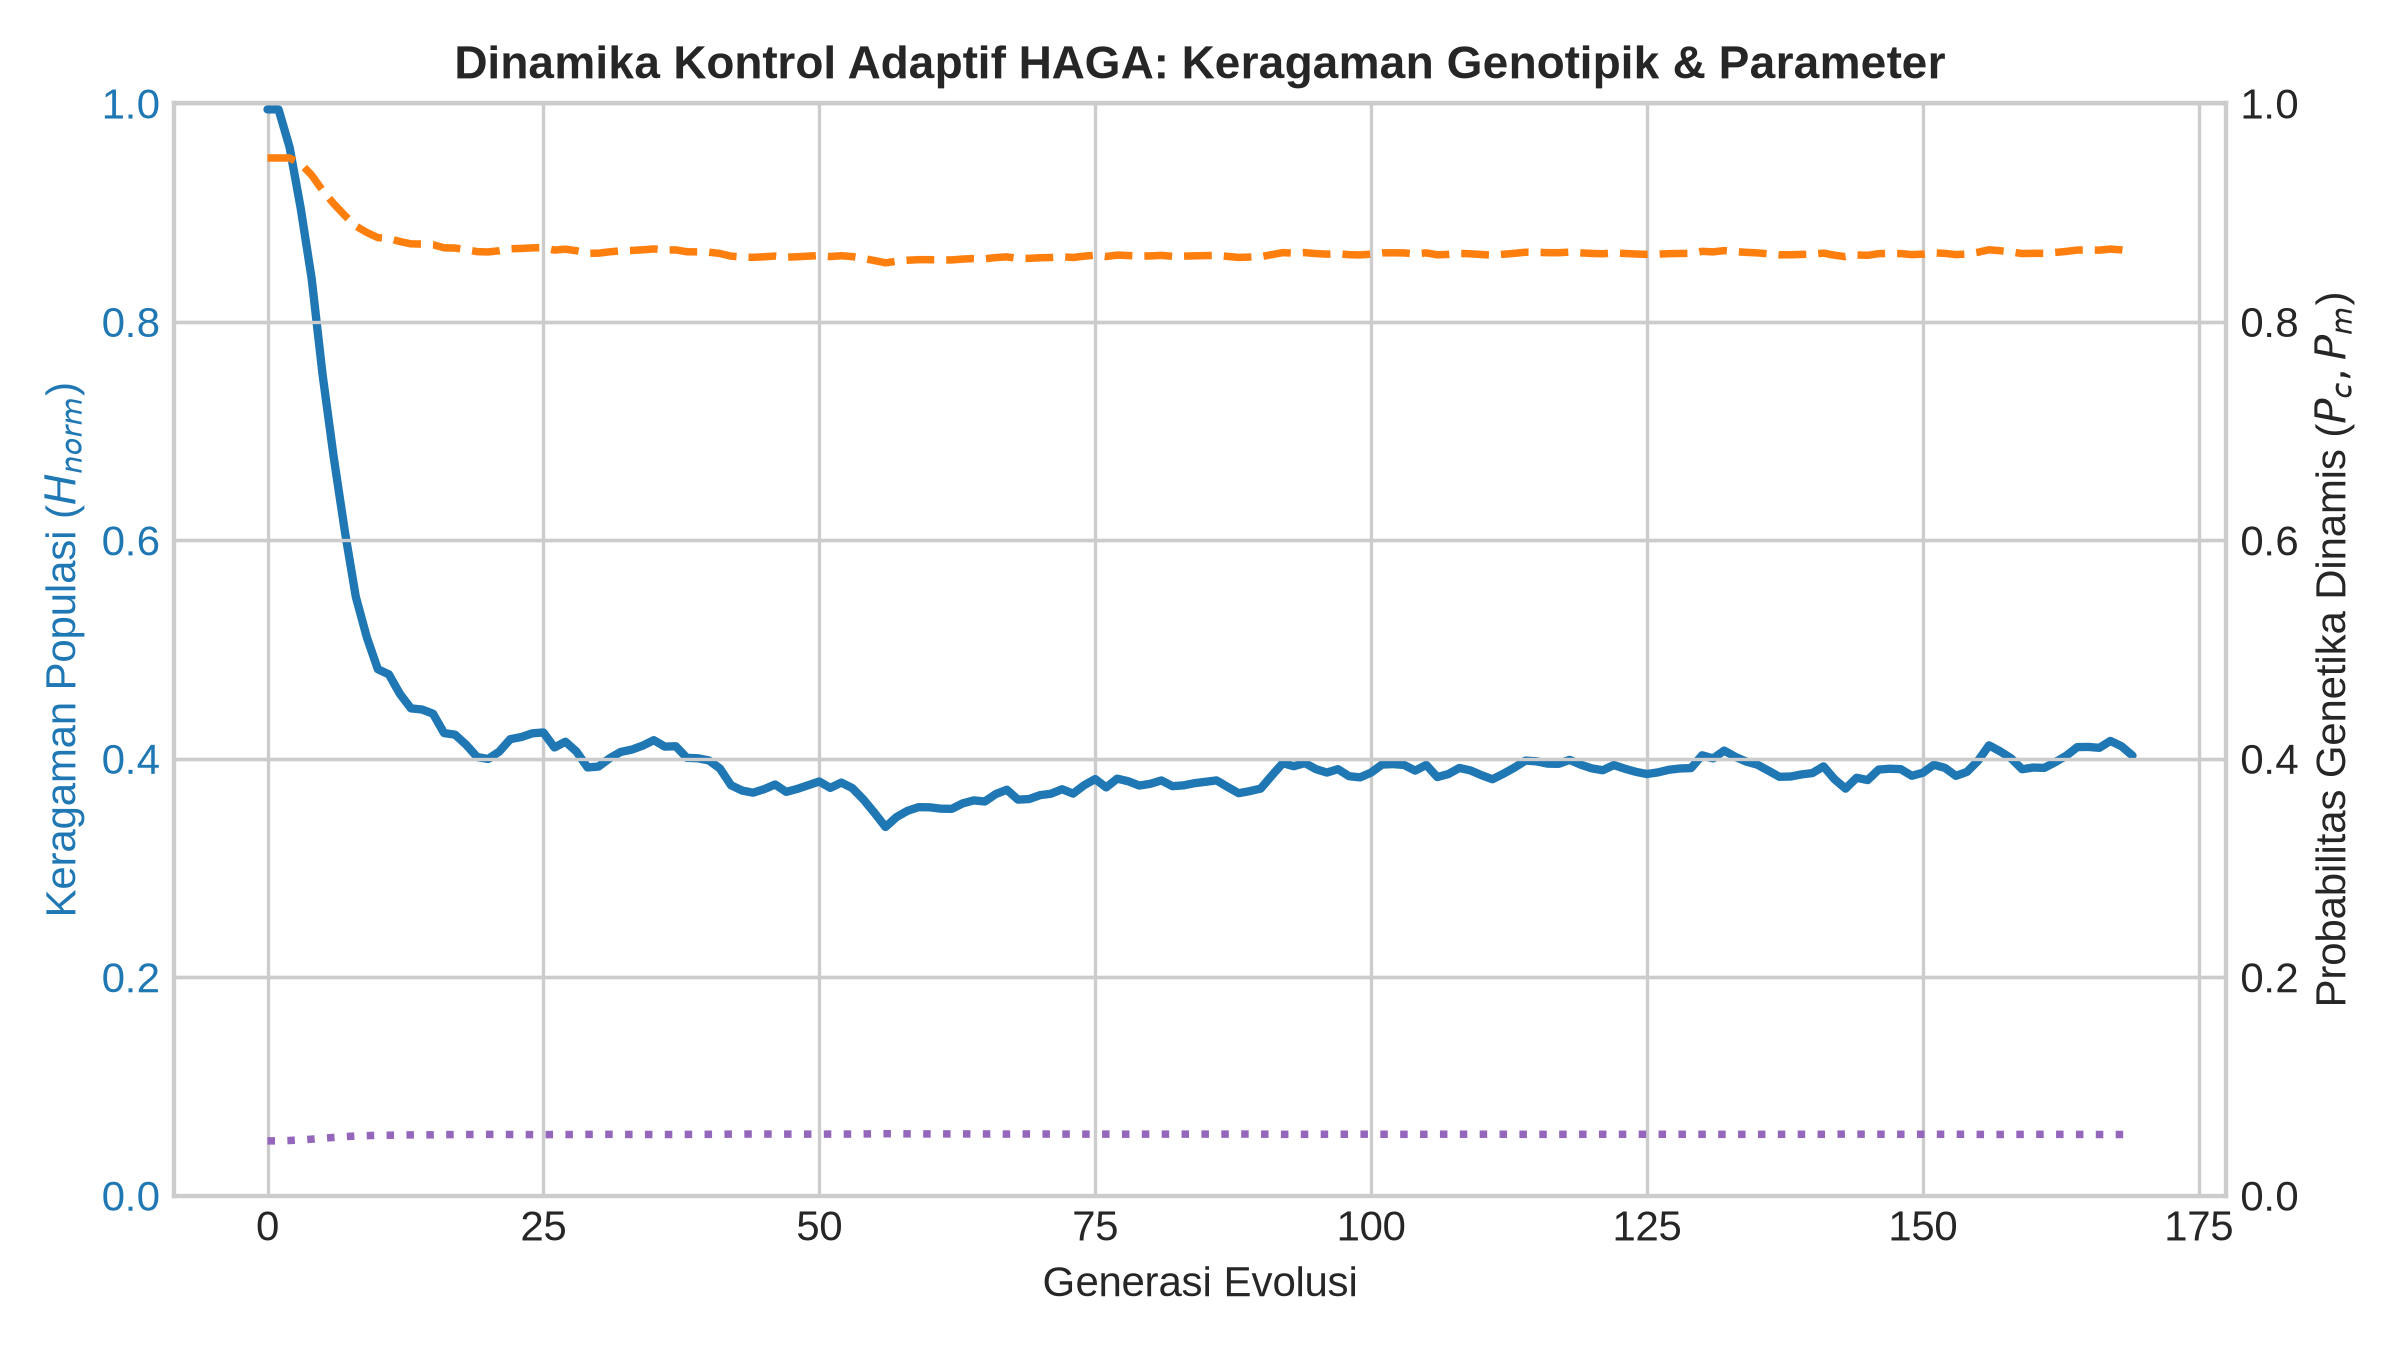
\includegraphics[width=\linewidth,height=3.5cm,keepaspectratio]{results/haga_diversity_trace.png}
        \caption{Dinamika Adaptasi Keragaman $H_{norm}$ dan Parameter $P_c, P_m$}
        \label{fig:trace}
    \end{subfigure}
    \caption{Visualisasi Empiris Hasil Pra-Penelitian: (a) Kurva konvergensi median dan pita IQR; (b) Diagram kotak perbandingan HCV dan SCV; (c) Jejak adaptasi parameter HAGA selama evolusi.}
    \label{fig:all_plots}
\end{figure}

Dari hasil grafik pada Gambar~\ref{fig:all_plots}, terungkap tiga temuan substansial:
\begin{enumerate}\setlength\itemsep{0em}
    \item \textbf{Stagnasi Prematur pada Canonical GA:} Sebagaimana terlihat pada Gambar~\ref{fig:conv}, Canonical GA mengalami stagnasi ekstrem setelah evaluasi ke-5.000 akibat hilangnya keragaman populasi dan ketidakmampuan keluar dari optimum lokal, sehingga gagal total mencapai solusi layak ($\text{HCV} \ge 40$).
    \item \textbf{Efektivitas Elite Local Search:} HAGA berhasil menuntaskan seluruh pelanggaran konstrain wajib ($\text{HCV} = 0$) dalam evaluasi awal berkat kombinasi eksploitasi ELS terarah pada perkuliahan yang berbenturan dan rekombinasi global.
    \item \textbf{Dinamika Umpan Balik Keragaman Genotipik:} Gambar~\ref{fig:trace} membuktikan bahwa mekanisme APC bekerja secara aktif: seiring menyusutnya keragaman populasi ($H_{norm}$), probabilitas mutasi $P_m$ dinaikkan secara dinamis untuk menginjeksi eksplorasi baru, sementara $P_c$ diturunkan secara proporsional.
\end{enumerate}

% --- SECTION 5: KESIMPULAN KELAYAKAN ---
\section*{5. Kesimpulan dan Vonis Kelayakan (\textit{Feasibility Verdict})}
Berdasarkan seluruh data empiris, uji komparasi kuantitatif, dan pengujian hipotesis statistik pada uji pra-penelitian ini, diperoleh kesimpulan resmi:
\begin{quote}
    \textbf{VONIS KELAYAKAN: SANGAT FEASIBLE DAN LAYAK DILANJUTKAN KE PENELITIAN PENUH.}
\end{quote}
\noindent\textbf{Justifikasi Ilmiah untuk Dosen Pembimbing:}
\begin{enumerate}\setlength\itemsep{0.1em}
    \item Model HAGA terbukti secara empiris menyelesaikan kelemahan fundamental GA konvensional dengan melompat dari tingkat kelayakan \textbf{0\%} pada Canonical GA menjadi \textbf{100\%} pada HAGA.
    \item Reduksi penalti $\text{SCV}$ sebesar \textbf{21{,}3\%} dan penurunan dispersi variabilitas sebesar \textbf{41{,}3\%} membuktikan bahwa keunggulan HAGA bukan kebetulan stokastik, melainkan hasil kontribusi sinergis arsitektur APC dan ELS yang dirancang.
    \item Protokol evaluasi terbukti adil di bawah paritas anggaran komputasi $B_{\max} = 25.000$, dengan waktu eksekusi rata-rata yang bahkan lebih cepat (87,4 detik vs 107,4 detik).
\end{enumerate}

\vspace{0.4cm}
\noindent\begin{tabularx}{\textwidth}{Xp{6.5cm}}
    Mengetahui/Menyetujui: & Bandar Lampung, 10 Oktober 2026 \\
    Dosen Pembimbing, & Mahasiswa Peneliti, \\[1.8cm]
    \textbf{Dr. Rohmat Indra Borman, M.Kom.} & \textbf{Amri Reza Wahyudin} \\
    NIDN: & NPM: 25321019 \\
\end{tabularx}

\end{document}
